%===============================================================================
% FETCH
%===============================================================================
% $Id$
%===============================================================================


%===============================================================================
% Configuration
%===============================================================================


%-------------------------------------------------------------------------------
% \documentclass and \usepackage directives
%-------------------------------------------------------------------------------
\documentclass[a4paper,fleqn]{report} 
%\usepackage{ngerman}
\usepackage[latin1]{inputenc}
\usepackage[T1]{fontenc}
\usepackage[small,hang,bf]{caption2}
\usepackage{fancyhdr}
\usepackage[nice]{nicefrac}
\usepackage{color,listings}
\usepackage{alltt}


% Compilation with latex or pdflatex?
\newif\ifpdf 
\ifx\pdfoutput\undefined 
  \pdffalse
\else
  \pdfoutput=1 
  \pdftrue 
\fi 

% Compilation with pdflatex
\ifpdf
 
  \usepackage[pdftex]{graphicx}

  \usepackage[
    pdftex,
    a4paper,
    bookmarks,
    pdfstartview=FitH,    % starts with page width
    bookmarksopen,        % opens index
    bookmarksnumbered,    % index with numbering
    colorlinks,           % links with color, otherwise with border
    linkcolor=blue,       % Standard red
    citecolor=blue,       % Standard green
    urlcolor=magenta,     % Standard cyan
    filecolor=blue
  ]{hyperref} 

  \pdfinfo{
    /Title      (FETCH)
    /Author     (Thomas Weibel)
    /Subject    (Eiffel programming)
    /Keywords   (Programming, Eiffel, Configuration)
  }

  % Use default Acrobat reader fonts
  \usepackage{mathpazo}

  % Use CM fonts (increases document size)
  % \usepackage{ae}

% Compilation with latex
\else 

  \usepackage{graphicx} 

\fi


%-------------------------------------------------------------------------------
% Configure \maketitle
%-------------------------------------------------------------------------------
\title{EiffelRSS \\ FETCH \\ Developer Guide}
\author{
  Michael K\"aser <kaeserm@student.ethz.ch>
  \and 
  Martin Luder <luderm@student.ethz.ch>
  \and 
  Thomas Weibel <weibelt@student.ethz.ch>
}
\date{\today}


%-------------------------------------------------------------------------------
% Configure fancyhdr
%-------------------------------------------------------------------------------
\pagestyle{fancy}

\renewcommand{\headrulewidth}{0.1 pt}
\renewcommand{\footrulewidth}{0.1 pt}

\fancypagestyle{plain}{
  \lhead{\nouppercase{\leftmark}}
  \chead{}
  \rhead{\thepage}
  \lfoot{FETCH}
  \cfoot{}
  \rfoot{Developer Guide}
}

\lhead{\nouppercase{\leftmark}}
\chead{}
\rhead{\thepage}

\lfoot{FETCH}
\cfoot{}
\rfoot{Developer Guide}


%-------------------------------------------------------------------------------
% Configure listings
%-------------------------------------------------------------------------------
\lstset{showstringspaces=false,
  breaklines=true,
  breakindent=0pt,
  prebreak=\mbox{\tiny$\searrow$},
  postbreak=\mbox{{\color{blue}\tiny$\rightarrow$}}}


%-------------------------------------------------------------------------------
% Common configuration
%-------------------------------------------------------------------------------
\setlength{\parindent}{0em}
\setlength{\parskip}{1.5ex plus0.5ex minus0.5ex}
\sloppy
\setlength{\mathindent}{0em}


%-------------------------------------------------------------------------------
% Commandos
%-------------------------------------------------------------------------------
\newcommand{\hr}{\rule{\textwidth}{1pt}}


%===============================================================================
% Document
%===============================================================================
\begin{document}

\begin{titlepage}
  \newlength{\centeroffset}
  \setlength{\centeroffset}{-0.5\oddsidemargin}
  \addtolength{\centeroffset}{0.5\evensidemargin}

  \thispagestyle{empty}

  \noindent
\includegraphics[width=\textwidth]{../../eth-logo/big_ETH}\\[-3mm]
  \hr

  \vspace*{\stretch{1}}

  \makebox[0pt][l]{
    \begin{minipage}{\textwidth}
      \flushright{
        \Huge\bfseries EiffelRSS
      }

      \noindent\rule{\textwidth}{3pt}\\[2.5ex]

      \hfill\emph{
        \Large FETCH: Developer Guide
      }
    \end{minipage}
  }

  \vspace{\stretch{1}}

  \makebox[0pt][l]{
    \begin{minipage}{\textwidth}
      \flushright{
        \bfseries 
        Michael K\"aser <kaeserm@student.ethz.ch>\\[0.3ex]
        Martin Luder <luderm@student.ethz.ch>\\[0.3ex]
        Thomas Weibel <weibelt@student.ethz.ch>\\[0.3ex]
      }
    \end{minipage}
  }

  \vspace{\stretch{1}}

  \noindent\hr\\[1mm]
  
\includegraphics[width=\textwidth]{../../eth-logo/big_inf}
\end{titlepage}

% Use roman page numbering
\pagenumbering{roman}

\begin{abstract}
  \texttt{FETCH} is a class which has features that can fetch data
  from a source address to a local \texttt{STRING} using various
  services.
  
  \texttt{FETCH} provides a simple interface for the
  \texttt{DATA\_RESOURCE} class in EiffelNet.
\end{abstract}

\clearpage
\tableofcontents

\clearpage
\listoffigures

\chapter{Introduction}
\label{cha:introduction}


% Set page counter to zero
\setcounter{page}{0} 

% Use arabic page numbering
\pagenumbering{arabic}


\section{Overview}
\label{sec:overview}

\texttt{FETCH} is a class which has features that can fetch data from
a source address to a local \texttt{STRING} using various services.
  
\texttt{FETCH} provides a simple interface for the
\texttt{DATA\_RESOURCE} class in EiffelNet.

A valid source address has the following format:
\texttt{service://address}.

Supported services are: file, http, ftp.

See figure \ref{fig:uml-diagram} for an overview of the class.

\begin{figure}[htbp]
  \centering
  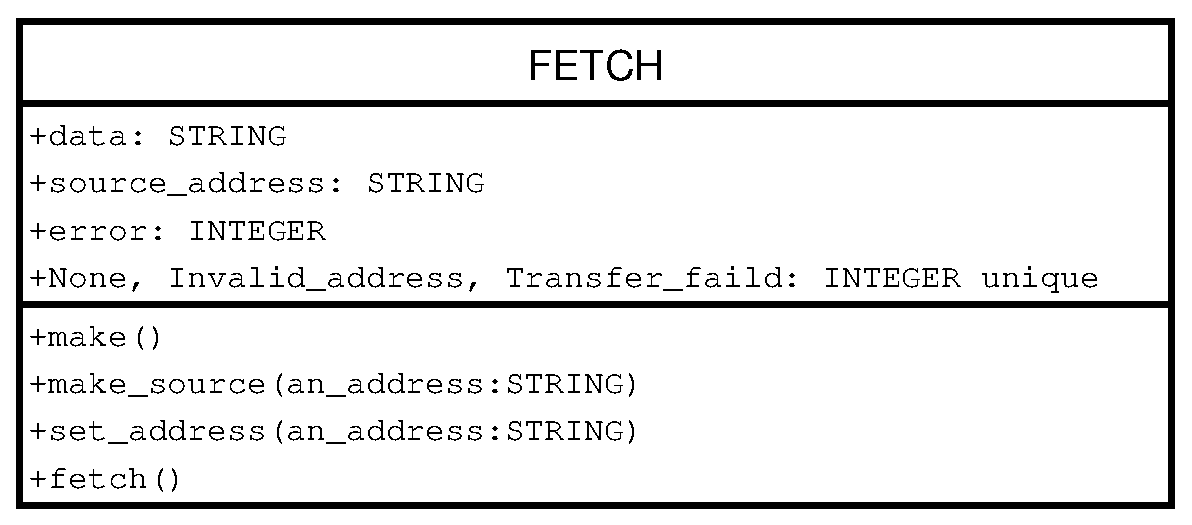
\includegraphics[width=\textwidth]{./figures/uml}
  \caption{UML diagram of \texttt{FETCH}}
  \label{fig:uml-diagram}
\end{figure}


\section{Usage}
\label{sec:usage}

\begin{lstlisting}[language=Eiffel]
class
  USAGE_EXAMPLE

create
  make

feature -- Initialization

  make is
      -- Creation procedure.
    local
      fetch: FETCH
      address: STRING
    do                          
      create fetch.make
                        
      io.put_string ("Please enter an address to fetch: %N")
      io.read_line

      address := io.last_string.twin

      fetch.set_address (address)
      fetch.fetch
                        
      io.put_new_line
                        
      if (fetch.error = fetch.Invalid_address) then
        io.put_string ("Error: Invalid address")
      elseif (fetch.error = fetch.Transfer_failed) then
        io.put_string ("Error: Transfer failed")
      else
        io.put_string (fetch.data)
      end

      io.put_new_line
  end

end -- class USAGE_EXAMPLE
\end{lstlisting}


\chapter{Features}
\label{cha:features}


\section{Initialization}
\label{sec:initialization}


\subsection{make}
\label{sec:make}

\begin{lstlisting}[language=Eiffel]
make ()
  -- Create the object without a source address
\end{lstlisting}


\subsection{make\_source}
\label{sec:make_source}

\begin{lstlisting}[language=Eiffel]
make_source (an_address: STRING) is
  -- Create the object with a predefined source
\end{lstlisting}


\section{Access}
\label{sec:access}


\subsection{data}
\label{sec:data}

\begin{lstlisting}[language=Eiffel]
data: STRING
  -- The data fetched
\end{lstlisting}

This can be void if there was an error.


\subsection{source\_address}
\label{sec:source_address}

\begin{lstlisting}[language=Eiffel]
source_address: STRING
  -- The source address
\end{lstlisting}

This can be void.


\subsection{error}
\label{sec:error}

\begin{lstlisting}[language=Eiffel]
error: INTEGER
  -- An error number
\end{lstlisting}

\texttt{error} can be one of the following constants: \texttt{None},
\texttt{Invalid\_address}, \texttt{Transfer\_failed}.

None means that there was no error and data is avaiable.
\texttt{Invalid\_address} means that the given source address was
either empty or not valid. If the error is \texttt{Transfer\_failed},
there was a problem when trying to load the data, i.e. there was no
connection to the internet.


\section{Basic Operations}
\label{sec:basic-operations}


\subsection{set\_address}
\label{sec:set_address}

\begin{lstlisting}[language=Eiffel]
set_address (an_address: STRING)
  -- Sets the address to an_address
\end{lstlisting}

This sets the source address to \texttt{an\_address}. After calling
this feature, \texttt{error} can be \texttt{Invalid\_address}.


\subsection{fetch}
\label{sec:fetch}

\begin{lstlisting}[language=Eiffel]
fetch
  -- Try to fetch the data from source_address
\end{lstlisting}

If \texttt{error} is not \texttt{Invalid\_address}, fetch tries to
open it and load the data. If there is a problem while loading the
data, \texttt{error} is set to \texttt{Transfer\_failed}.

\end{document}
